%!TEX root=main.tex

\subsection{Manual de utilização}

\subsubsection{Vers\~ao Consola}

Na pasta ``CODIGO SOURCE'' está disponível quase todo o código desenvolvido para o projeto. Esta n\~ao inclui código para a interface gráfica nem testes manuais realizados pela equipa. No ficheiro Program.cs já se encontram duas funções relativas às experiências efetuadas comentadas. Para corre-las é preciso descomentá-las e compilar o código. Para especificar mais concretamente os testes a correr em vez de apenas usar estas linhas de código presentes no Program.cs ou para fazer uso de outras funcionalidades implementadas é necessário estar familiarizado com a \verb|framework| implementada. 

Se desejar compilar e correr esta versão do código pode usar uma versão do ~\verb|Visual Studio| que suporte C\#. Pode criar um novo projeto para consola em C\# e arrastar os ficheiros manualmente para a pasta de projeto. Depois de arrastados é necessário inclui-los no projeto criado a partir do ~\verb|Solution Explorer|. As imagens seguintes ilustram como pode realizar esta última etapa. Caso pretenda usar a ferramenta sugerida pode consultar o ~\href{https://msdn.microsoft.com/en-us/library/aa187916.aspx}{MSDN} em caso de dúvidas. Alternativamente também pode optar por usar o ~\href{http://www.mono-project.com/docs/about-mono/languages/csharp/}{Mono}.

\begin{table}[H]
\centering
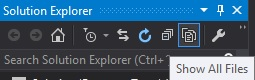
\includegraphics[height=3cm]{user_manual/showallfiles.jpg}
\end{table}

\begin{table}[H]
\centering
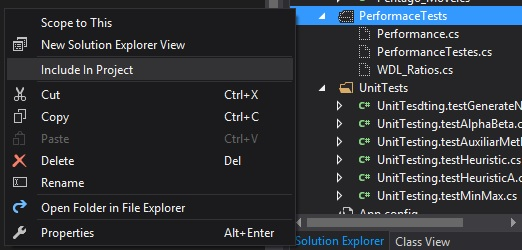
\includegraphics[height=4cm]{user_manual/includestuff.jpg}
\end{table}

\begin{table}[H]
\centering
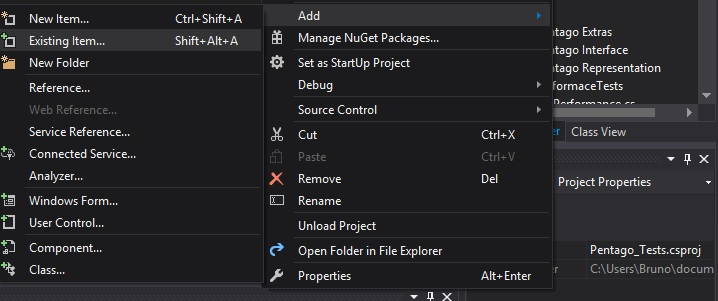
\includegraphics[height=4cm]{user_manual/includestuff2.jpg}
\end{table}

\newpage
\subsubsection{Vers\~ao Unity}

No ``PentagoLastBuildAndSource.rar'' contem uma pasta denominada ``PENTAGO\_ALL'' onde encontram-se outras duas pastas. 

Uma pasta denominada de ``Pentago\_LastBuild'' contem o projeto já compilado para correr em browser independentemente do sistema operativo usado. Para correr esta versão do jogo com interface gráfica deve usar um browser que tenha instalado o ~\href{https://unity3d.com/pt/webplayer}{plugin do Unity}. 

Uma outra pasta denominada de Pentago contem o projeto Unity com todo o código, modelos e conteúdo usado no desenvolvimento. O código desenvolvido especificamente para esta versão encontra-se dentro de ``Assets\\Scripts''. Além das componentes ligadas ao interface gráfico também é possível reparar em mudanças mínimas no código original. Caso pretenda editar ou compilar necessita de uma vers\~ao do Unity compatível com o mesmo (em principio todas as versões 5.x deverão funcionar). Para abrir o projeto abra uma ~\verb|scene| do mesmo e para compilar é necessário que as ~\verb|scenes| estejam incluídas nos ~\verb|Build Settings|. As figuras seguintes ilustram estas etapas. Note que pode optar por compilar para um sistema operativo em vez de browser.

\begin{table}[H]
\centering
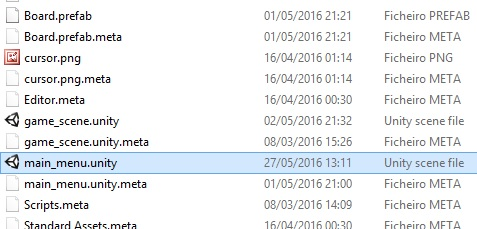
\includegraphics[height=5cm]{user_manual/unityscene.jpg}
\end{table}

\begin{table}[H]
\centering
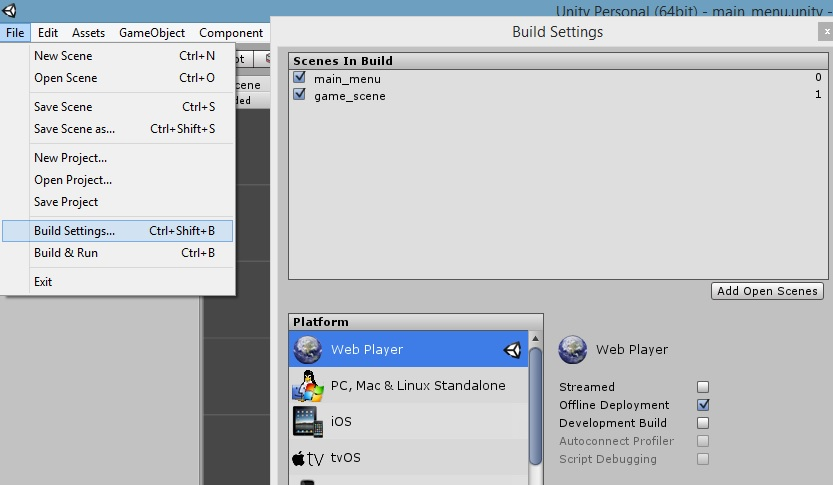
\includegraphics[height=8cm]{user_manual/unitybuild.jpg}
\end{table}

\newpage
\subsubsection{Notas relativas ao Jogo}

O jogo presenta uma naveç\~ao intuitiva e é bastante auto-explicativo. O único detalhe que talvez seja importante referir é que quando é usado o modo ``IA vs IA'' as ``\verb|IA setings|'' são sempre aplicadas às IA de peças brancas e as de ``\verb|2nd IA|'' à IA de peças pretas. Quando se joga no modo humano contra computador, independentemente das peças com que o jogador humano joga, o computador utiliza sempre as configurações definidas em \verb|IA setings|. Este detalhe n\~ao está explicito no interface gráfico e será adicionado posteriormente à entrega para esclarecimento dos utilizadores.

\begin{table}[H]
\centering
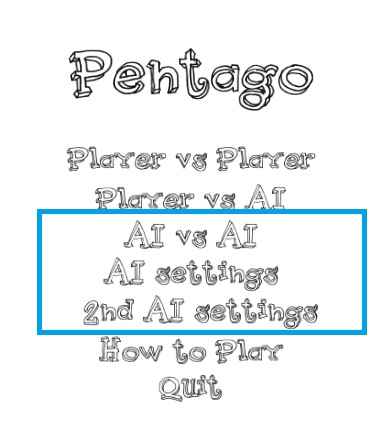
\includegraphics[height=8cm]{user_manual/iasettings.jpg}
\end{table}

Detalhes relativos a como jogar o jogo est\~ao descritos no próprio interface gráfico na secç\~ao ``\verb|How to Play|''.

